\documentclass[10pt,a4paper]{article}

\usepackage[english]{babel}
\renewcommand*\ttdefault{txtt}
\usepackage[T1]{fontenc}

\usepackage[round,authoryear]{natbib}

\usepackage[hidelinks]{hyperref}

\usepackage{graphicx}
\graphicspath{{./images/}}
\usepackage{todonotes}

\usepackage{listings}
\lstdefinelanguage{scala}{
  morekeywords={abstract,case,catch,class,def,do,else,extends,false,
                final,finally,for,if,implicit,import,match,mixin,new,
                null,object,override,package,private,protected,
                requires,return,sealed,super,this,trait,true,try,
                type,val,var,while,with,yield},
  otherkeywords={=,=>,<-,<\%,<:,>:,\#,@},
  sensitive=true,  
  morecomment=[l]//,
  morecomment=[n]{/*}{*/}, %or [s]
  morestring=[b]",
  morestring=[b]',
  morestring=[b]"""
}
\lstset{
  language=scala,
  showstringspaces=false,
  numbers=left,
  columns=fixed,
  breaklines=true,
  captionpos=t,
  basicstyle={\footnotesize\ttfamily}
}

\renewcommand\appendix{\par
\setcounter{section}{0}%
\setcounter{subsection}{0}%
\setcounter{table}{0}
\setcounter{figure}{0}
\setcounter{equation}{0}
\gdef\thetable{\Alph{table}}
\gdef\thefigure{\Alph{figure}}
\gdef\theequation{\Alph{section}-\arabic{equation}}
\section*{Appendix}
\gdef\thesection{\Alph{section}}
\setcounter{section}{0}}

\title{Visualizing Project Relations on GitHub}
\author{
    Hendrik van Antwerpen\\{\small\href{mailto:H.vanAntwerpen@student.tudelft.nl}{\nolinkurl{H.vanAntwerpen@student.tudelft.nl}}}
  \and
    Niels van Kaam\\{\small\href{mailto:N.vanKaam@student.tudelft.nl}{\nolinkurl{N.vanKaam@student.tudelft.nl}}}
}
\date{Software Engineering Research Group, EECMS\\Delft University of Technology}

\begin{document}

\maketitle

\begin{abstract}
GitHub has emerged as an interesting object of study for software repository analysis because of the data available through its open API. Visualizing this data can be challenging, because of the lack of knowledge about its structure and because of the size of the dataset. For distributed processing of large data sets functional programming techniques and models like MapReduce have become increasingly popular. In this report we describe a web based system that makes it possible to explore one type of relation in GitHub; the links between projects based on common committers. Users can explore the data by selecting time limits and minimum link weight. This report describes the implementation of that system in the object-oriented function programming language Scala, using Sawzall style aggregators and other functional programming techniques.
\end{abstract}

\section{Introduction}

In the field of software repository mining, GitHub has emerged as an interesting subject of study. Tools have emerged to collect and publish the data that GitHub exposes \citep{gousios2012ghtorrent}. Making sense of the data and visualizing it in interesting ways is not trivial. Finding interesting correlations and metrics is hard. Interactive software that visualizes aspects of the data while the user can influence constraints like time period or project language allows easy exploration of the data and can be a starting point for more formal analysis.

We present a web based software system that allows a user to explore relations between projects on GitHub. A relation is defined by the existence of a common committer. The user can influence the time period wherein the link must exists, the main programming language of the project and the minimum number of committers before a link is shown.

We identify several challenges in the design of the software:
\begin{itemize}
    \item Providing a general visualization that might reveal interesting properties of the data to the user.
    \item Dealing with the large size of the data that is being processed.
    \item Ensuring responsiveness and reduce waiting times of the software to encourage the user to explore.
\end{itemize}

The software was developed in the context of a functional programming course\footnote{\url{http://swerl.tudelft.nl/bin/view/Main/FunctionalProgrammingCourse}} at the Delft University of Technology. The course focused on functional programming techniques, application of these techniques in more imperative languages and using them for processing large data sets. The report therefore also describes how the functional programming and data processing techniques from the course were applied. The project was implemented using Scala and the code samples will be mostly in that language.

The report is structured as following:
\begin{itemize}
    \item A description of the data and the data processing (section \ref{sec:data}).
    \item A description of a MapReduce implementation in Scala, created to implement the data processing (section \ref{sec:mapreduce}).
    \item A description of the distributed design of the backend, created to improve responsiveness of the software (section \ref{sec:distributed}).
    \item A description of the visualization used in the web interface (section \ref{sec:visualization}).
    \item Conclusions and ideas for further research and development (section \ref{sec:conclusions}).
\end{itemize}

\section{Data set and processing strategy}\label{sec:data}

The raw data available was a list of projects and their main programming language, a list of users and a list of commits. A commit provides the basic link between a user and a project at a certain time. A link between projects exists when the have a common committer. We define the weight of a link to be the number of common committers and the weight of a project to be its degree, i.e. the number of projects it is connected to. Table \ref{tbl:dataset-numbers} lists some numbers on the data set. The distribution of unique project-user links per week is shown in figure \ref{fig:user-project-links-per-week}. Figure \ref{fig:link-weight-hist} shows a histogram of link weight. A histogram of the number of projects per user is shown in figure \ref{fig:projects-per-user-hist}.

\begin{table}
    \centering
    \begin{tabular}{l r}
        \hline
        \#projects & ~850k \\
        \#users & ~750k \\
        \#commits & ~14m \\
        \#unique project-user links per week & ~3m \\
        \#project links & 11m \\
        \hline
    \end{tabular}
    \caption{Some numbers about the data set}
    \label{tbl:dataset-numbers}
\end{table}

\begin{figure}[htb]
    \centering
    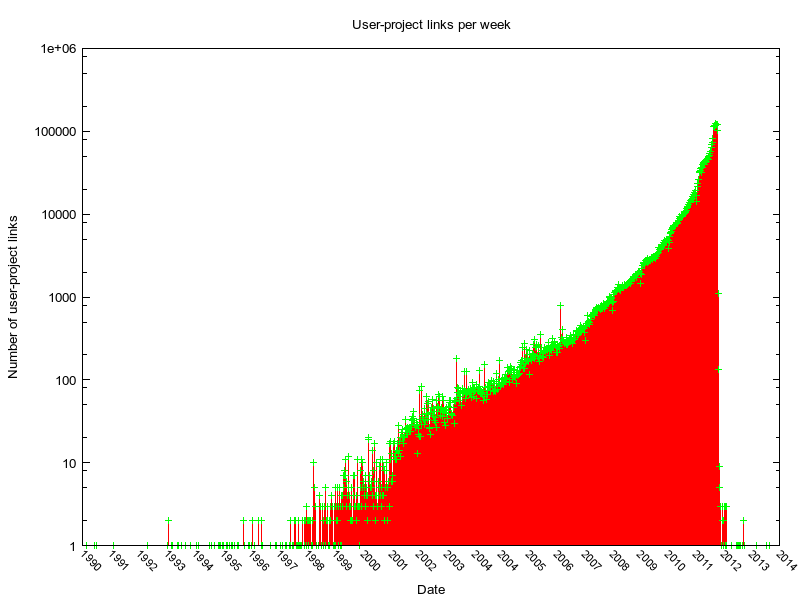
\includegraphics[width=0.75\textwidth]{user-project-links-per-week}
    \caption{Unique user-project links by week}
    \label{fig:user-project-links-per-week}
\end{figure}

\begin{figure}[htb]
    \centering
    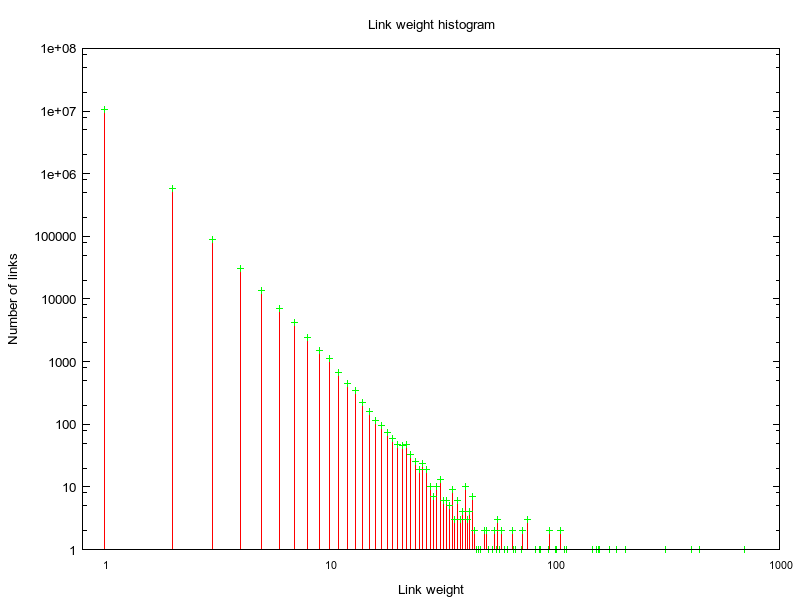
\includegraphics[width=0.75\textwidth]{link-weight-histogram}
    \caption{Link weight histogram}
    \label{fig:link-weight-hist}
\end{figure}

\begin{figure}[htb]
    \centering
    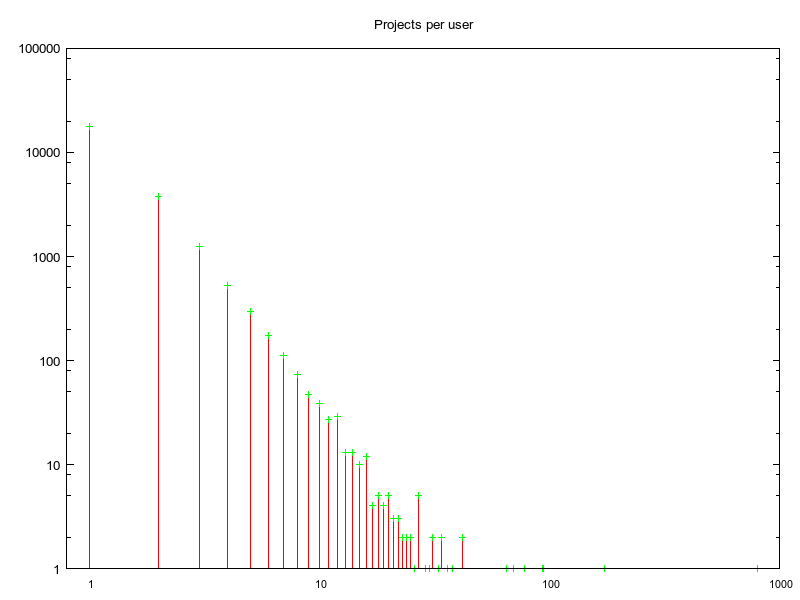
\includegraphics[width=0.75\textwidth]{projects-per-user-histogram}
    \caption{Projects per user histogram}
    \label{fig:projects-per-user-hist}
\end{figure}

We allow the user to vary the following parameters:
\begin{itemize}
    \item Time period.
    \item Minimum weight of a link before it's included.
\end{itemize}
The desired end result is a list of links between projects, the weight of each link and the weight of each project. This last property can identify central projects in the graph.

Processing data can be elegantly expressed as a stream of filter and transform operations. Without considering implementation details, those steps will be:
\begin{enumerate}
    \item Filter commits and exclude commits outside of the selected time period or not in the filtered project list.
    \item Build a set of projects per user.
    \item For each user's projects, create links between those projects.
    \item Merge project links, assigning them weight based on their occurrence.
    \item Transform the list of links to a format understood by the visualization code.
\end{enumerate}

\section{MapReduce with Scala collections}\label{sec:mapreduce}

An increasingly popular model for processing big data sets is MapReduce \citep{dean2008mapreduce}. This model lends itself well for distribution and parallel data processing. One descendant of this model is found in Google's Sawzall \citep{pike2005interpreting}, using aggregators as a key abstraction. In \cite{lammel2008google} a rigorous description of these two models is provided. The Sawzall concept of aggregators is identified as a generalized form of monoids. Their properties allow easy combination of parallel computed partial results, possible in a hierarchical way. Because monoids for common data types like lists, maps and tuples are readily available, developers need think less about the reduction of intermediate results and can focus on the map part of the process.

Sawzall is very liberal in the output it accepts from map functions. The output can be a monoid, a collection of the monoid or an element if the monoid is a collection itself. To capture all these, L\"ammel defines aggregators as generalized monoids:
\begin{lstlisting}[language=haskell]
class Monoid m => Aggregator e m | e -> m
  where
    minsert :: e -> m -> m
\end{lstlisting}

To our knowledge no implementation of this approach is available in Scala. Therefore we implemented a version of aggregators for Scala and used those to implement a map-reduce function that integrates seamless with the Scala collection library.

\subsection{Aggregators}

To implement the Sawzall model, we will start with the key abstraction, the aggregator. An aggregator is defined by the following trait:
\begin{lstlisting}
trait Aggregator[A,B] {
  def zero: A
  def insert(a: A, b: B): A
}
\end{lstlisting}
Because there is no readily available monoid type in Scala and we will use aggregators only, we dropped the requirement that type \lstinline|A| has to be a monoid. We use the term monoid aggregator for any \lstinline|Aggregator| where \lstinline|A| and \lstinline|B| are the same type, because this behaves the same as a monoid of that type would.

We defined the \lstinline[language=haskell]|minsert| function in Scala as \lstinline!a:A |<| b:B : A!. Whenever this operator is used, the compiler infers which \lstinline|Aggregator[A,B]| to use. All Scala \lstinline|implicit| rules apply, so if no \lstinline|Aggregator| is found there's compile time error. If multiple options are found the programmer has to specify manually which one to use.

We started with a basic monoid aggregator for sums, which serves as the default aggregator for integers in the rest of the examples. The implementation looks like:
\begin{lstlisting}
implicit def SumMonoid =
  new Aggregator[Int,Int] {
    override def zero = 0
    override def insert(a: Int, b: Int) = a + b
  }
\end{lstlisting}

The next step is implementing collection aggregators. Generally every collection type has two aggregators. One for the monoid case and one for the element insert case. For the case of lists, the signatures look like
\begin{lstlisting}
implicit def ListMonoid: Aggregator[List[A],List[A]] = ...
implicit def ListAggregator: Aggregator[List[A],A] = ...
\end{lstlisting}

Implementing this for a lot of collection types would be a daunting task. Luckily the design of the generic Scala collections library \citep{odersky2009fighting} comes to great help here. By using the \lstinline|CanBuildFrom[Coll,Elem,Result]| infrastructure and higher-order generics, we only have to implement two aggregators for any kind of \lstinline|GenSet|, for any kind of \lstinline|GenSeq| and for any kind of \lstinline|GenMap|.

As an example, lets look at the aggregators for \lstinline|GenSeq|, shown in listing \ref{lst:seq-aggregators}. The two cases (monoid and element) are implemented separately. Although the implementation is relatively straightforward, some things are note-worthy. In the monoid case, we are more liberal in our input than the type we produce. Every collection implements the \lstinline|GenTraversableOnce[A]| interface for it's element types and allows easy appending of such a collection. Apart from the case \lstinline!List[Int] |<| List[Int]! this also allows us to do things like \lstinline!List[Int] |<| Set[Int]!. Apart from being liberal in the collection type we insert, we are also covariant in the collections element type. This is intuitive for programmers, when a collection takes elements of type \lstinline|A|, one can also insert elements of a subtype \lstinline|B <: A|. Because type inferences considers the type \lstinline|Elem| to be invariant, we added the extra \lstinline|InElem <: Elem| to allow any subtype as well.

\begin{lstlisting}[float,frame=tb,caption=Aggregators for sequences,label=lst:seq-aggregators]
implicit def GenSeqAggregator[Repr[X] <: GenSeq[X], Elem, InElem <: Elem]
                             (implicit bf: CanBuildFrom[Nothing,Elem,Repr[Elem]]) =
  new Aggregator[Repr[Elem],InElem] {
    override def zero: Repr[Elem] = bf().result
    override def insert(s: Repr[Elem], e: InElem) =
      (s :+ e).asInstanceOf[Repr[Elem]]
  }

implicit def GenSeqMonoid[Repr[X] <: GenSeq[X], Elem, In[X] <: GenTraversableOnce[X], InElem <: Elem]
                         (implicit bf: CanBuildFrom[GenSeq[Elem],Elem,Repr[Elem]]) =
  new Aggregator[Repr[Elem],In[InElem]] {
    override def zero: Repr[Elem] = bf().result
    override def insert(s1: Repr[Elem], s2: In[InElem]) =
      (s1.++(s2)(bf))
  }
\end{lstlisting}

For \lstinline|Map| there was some extra work to be done. Although \lstinline|Map[K,V] <: Traversable[(K,V)]| the compile would not infer the aggregator when a map was provided, like \lstinline!Map[Int,Int] |<| Map[Int,Int]!. Therefore another monoid aggregator was implemented for this specific case, although still general for any \lstinline|Map| type.

This brings the count for our collection aggregators to seven and covers all cases. Some examples to show what we can do with it:
\begin{lstlisting}
// Int |<| Int : Int
1 |<| 2 // = 3

// List[Int] |<| Set[Int] : List[Int]
List(1,2) |<| Set(3) // = List(1,2,3)

// SortedSet[Int] |<| Int : SortedSet[Int]
SortedSet(2,3) |<| 1 // = SortedSet(1,2,3)

// simple word count coming up!
// Map[String,Int] |<| (String,Int) : Map[String,Int]
Map("aap"->1,"noot"->2) |<| ("noot",1) // = Map("aap"->1,"noot"->3)
\end{lstlisting}

A nice property of monoids is that they can be structurally combined. For example a tuple with two monoid values is itself a monoid. In our aggregator world, we happen to have similar properties. Aggregators for \lstinline|TupleN| (see listing \ref{lst:tuple-aggregator}) and \lstinline|Map| where implemented to require their tuple values and map value to be aggregators themselves. This is a difference with L\"ammels description, where the nested values are strict monoids. Our approach introduces a lot of flexibility in the elements that can be inserted. When creating deep structures, on every level we have the choice to insert either a value or a collection. Some examples should show the flexibility this gives us:
\begin{lstlisting}
// count individual and total words
// (Int,Map[String,Int]) |<| (Int,(String,Int)) : (Int,Map[String,Int])
(3,Map("aap"->1,"noot"->2)) |<| (1,("aap",1)) // = (4,Map("aap"->2,"noot"->2))

// or (Int,Map[String,Int]) |<| (Int,Map[String,Int]) : (Int,Map[String,Int])
(1,Map("aap"->1)) |<| (3,Map("aap"->1,"noot"->2)) // = (4,Map("aap"->2,"noot"->2))
\end{lstlisting}

\begin{lstlisting}[float,frame=tb,caption=Aggregator for tuple,label=lst:tuple-aggregator]
implicit def Tuple2Aggregator[A1,A2,B1,B2]
             (implicit a1: Aggregator[A1,B1],
                       a2: Aggregator[A2,B2]) =
  new Aggregator[(A1,A2),(B1,B2)] {
    override def zero = (a1.zero,a2.zero)
    override def insert(a: (A1,A2), b: (B1,B2)) =
      (a1.insert(a._1, b._1),a2.insert(a._2, b._2))
  }
\end{lstlisting}

One aspect of the Sawzall aggregators is not addressed yet: the possibility to insert a collection of elements. For this case we implemented an aggregator similar to L\"ammel's \lstinline[language=haskell]|Group| aggregator, shown in listing \ref{lst:group-aggregator}. Note that this works again at every level of nested types, so this allows us to do things like:
\begin{lstlisting}
// Int |<| List[Int] : Int
3 |<| List(2,5) // = 10

// Map[Int,Int] |<| List[(Int,List[Int])] : Map[Int,Int]
Map(1->1) |<| List((1,List(2,3)),(7,List(42))) // = Map(1->6,7->42)
\end{lstlisting}

\begin{lstlisting}[float,frame=tb,caption=Aggregator for collections of elements,label=lst:group-aggregator]
implicit def GroupAggregator[Coll,In[X] <: GenTraversableOnce[X],Elem]
                            (implicit va: Aggregator[Coll,Elem])=
  new Aggregator[Coll,In[Elem]] {
    override def zero = va.zero
    override def insert(a: Coll, as: In[Elem]) =
      (a /: as)( (c,e) => va insert (c,e) )
  }
\end{lstlisting}

Our design allows a lot of freedom in the shape of the elements inserted into a collection. What type of elements can be inserted is dictated by the defined aggregators and fully inferred by the compiler. The aggregators for the Scala collections are very generic and in most cases the developer doesn't have to care about how to merge collections. Monoid aggregators are implemented for string concatenation and integer summing, but others are very easy to implement; one implicit function and an implementation of the \lstinline|Aggregator| trait is enough.

\subsection{MapReduce}

Using the developed aggregators, a map-reduce library was implemented. We want the map-reduce functionality to be as easy to use as the standard collection functions like \lstinline|map| or \lstinline|filter|. To a high degree this can be achieved by enriching libraries, a process similar to defining type classes in Haskell (see \cite{odersky2006pimp} for details).

Using again the generic design of the collections library and type inference allows us to write map-reduce by only specifying the expected result type. The full implementation is shown in listing \ref{lst:map-reduce}. Our first implementation defined \lstinline|def mapReduce[ResultColl,ResultElem](f: Elem => ResultElem)|. Unfortunately it is not possible in Scala to provide some of the type parameters but have others inferred. This forced us to repeat the return type of the function when specifying the result type of the \lstinline|mapReduce| call. Introducing the intermediate \lstinline|MapReducer| object solved this problem. The result type of mapReduce was specified on the call, but the return type of the function could be inferred for the \lstinline|apply| call. Because parentheses can be omitted when a function has no arguments, this resulted in a syntax identical to a case without the intermediate object, but with one less type parameter. A word count example similar to one L\"ammel gives now looks like:
\begin{lstlisting}
val docs: List[String] = ...
def wordcount(doc: String): List[(String,Int)] = doc.split(" ").toList.map( w => (w,1) )
val wc = docs.mapReduce[Map[String,Int]]( wordcount )
\end{lstlisting}

\begin{lstlisting}[float,frame=tb,caption=MapReduce for Scala collections,label=lst:map-reduce]
object MapReduce {

  class GenMapReducer[Elem](as: GenTraversableOnce[Elem]){
    def mapReduce[ResultColl] = new MapReducer[ResultColl]
    class MapReducer[ResultColl] {
       def apply[ResultElem](f: Elem => ResultElem)
                (implicit p: Aggregator[ResultColl,ResultElem])
                : ResultColl =
  	     (p.zero /: as)( (c,a) => p.insert(c, f(a)) )
    }
  }

  implicit def mkMapReducable[Elem](as: GenTraversableOnce[Elem]) =
    new GenMapReducer[Elem](as)

}
\end{lstlisting}

The performance of our map-reduce is in the range as hand written code using e.g. \lstinline|foldLeft|. Most of the work is done through inference by the compiler. At runtime the aggregators use folds and collection operations just as you would in handwritten code. There a little overhead of some function calls, but all the reduction details are abstracted away, resulting in less repetition and simpler data transformation functions.

It is possible that multiple aggregators for the same type exist, for example a sum and a product on numbers. In such a case it is very easy to specify which one to use. Here is a small example:
\begin{lstlisting}
def SumMonoid: Aggregator[Int,Int] = ...
def ProductMonoid: Aggregator[Int,Int] = ...

val words: List[String] = ...
val sumOfWordLengths = words.mapReduce( w => w.size )(SumMonoid)
val prodOfWordLengths = words.mapReduce( w => w.size )(ProductMonoid)
\end{lstlisting}
As you can see the result type is not required, because it is inferred from the aggregator.

This fully implements the Sawzall map-reduce model as it is formalized in \cite{lammel2008google}. The use of aggregators instead of monoids gives us even more freedom in the output of our map functions than L\"ammel's model does. The integration with the Scala collections library makes using map-reduce very easy for programmers used to that idiom.

With all pieces in place, we can write our processing steps from section \ref{sec:data} in Scala:
\begin{lstlisting}
val commits: List[Commit] = ...
def projectsToPairs(ps: List[Project]): List[(Project,Project)] = ...
val linkMap = 
  commits.filter( c => c.timestamp >= from && c.timestamp <= until  )
         .mapReduce[Map[User,Set[Project]]]( c => (c.user,c.project) )
         .values
         .mapReduce[Map[(Project,Project),Int]](projectsToParis)
         .filter( _._2 >= minWeight )
\end{lstlisting}

\section{Distributed data-processing with Akka}\label{sec:distributed}
Even tough the computation of the project links has been optimised,  a lot of data needs to be processed; Our dataset consists of 14 million commits. Because of this a request on a set of project links for a given time-interval and weight could take around 2 minutes for the entire dataset. This might be enough to compute a single graph, but for interactive use this is not acceptable. Therefore we decided to distribute the computation by using actors. Because the system was built in Scala, the most logical choice for this is using the Akka toolkit, which is the most commonly used actor toolkit for Scala.

\subsection{Akka}

Akka is a toolkit for, as they state themselves, "building highly concurrent, distributed event driven applications". The main parts in Akka that were used for the distribution are the "Actors" and "Futures". In Akka actors are created on a "actor system", and actors communicate by sending messages between each other. Actor systems running on separate hosts can also be combined to work as one actor system. When the system is configured properly each actor reference is "network aware", meaning that it can be passed from one actor system to another while the reference remains intact. For the actors this means it does not matter where other actors are located physically.

When using multiple actors, computations will be done asynchronous. One way to deal with this asynchronous time is to use the Akka "Futures" and the "Ask" pattern. When using the Ask pattern, the result of a "Ask" message to an actor can be stored in a future. A future is a monad, which will eventually obtain the value an actor is computing. This means that while the result is not available yet other functions can be mapped over the future, to be computed when the result becomes available. 

A future can also be piped to an actor, meaning that when the result becomes available, all operations over the future will be executed, and the result will be sent as message to the actor the future was piped to. This way an entire computation chain can be composed which will automatically completed when the results become available.

What Akka actually does behind the scenes for each future obtained by an ask request is creating a new actor, which reacts on the "reply message". When the reply message is sent the operations that were mapped over the future are executed, and the result is send to the actor the future was piped to. This can also be seen in figure \ref{fig:actor_seq}, which will be explained later.

\subsection{Distribution}

In order to reduce the total computation time by distributing the data over multiple actors, the data needs to be cut into multiple parts. Randomly cutting the dataset in multiple pieces is not possible in this case. A link between a project is defined as a "common committer". By splitting the dataset and computing one half on one actor and the other half on a second actor could cause these common commits to be broken. 

Therefore we came up with the following solution. We initially give each actor system access to the entire dataset. Then, when an computation-actor is created, it receives a set of users for whose commits it is responsible. We distribute the commits in a round robin fashion over the actors based on userid. With a set of users the actor can compute the entire process towards the project links, except for the filtering on the weight of the link. For that last operation an actor needs to be sure that it has all links between a project in order to produce a correct result. This is done at the highest level of the computation hierarchy when all links are available.

The computation-actors described above will send the project-links to the actor that sent the request (using the "Ask" pattern). This actor (the link-combiner-actor) receives them in a future, over which a reduction is mapped. The result of the future is piped to the actor that requested the links to the link-combiner-actor. This completes the computation chain.

To get the entire system working, two more actors are added. First is the webservice-actor which function is to handle requests from the user. For each request from the user, it "Asks" the link-combiner-actor for the project-links, and pipes the result to the JSON-converter-actor. The JSON-converter-actor is responsible for converting the list of  project links into a JSON format that can be parsed by the visualisation tool. Upon receiving a list of project-links the JSON-converter-actor converts the list into a JSON format and sends the result to the user. The resulting system is shown schematically in figure \ref{fig:actor_sample}. The communication between the actors and futures is shown a sequence diagram in figure \ref{fig:actor_seq}.

\begin{figure}[htb]
    \centering
    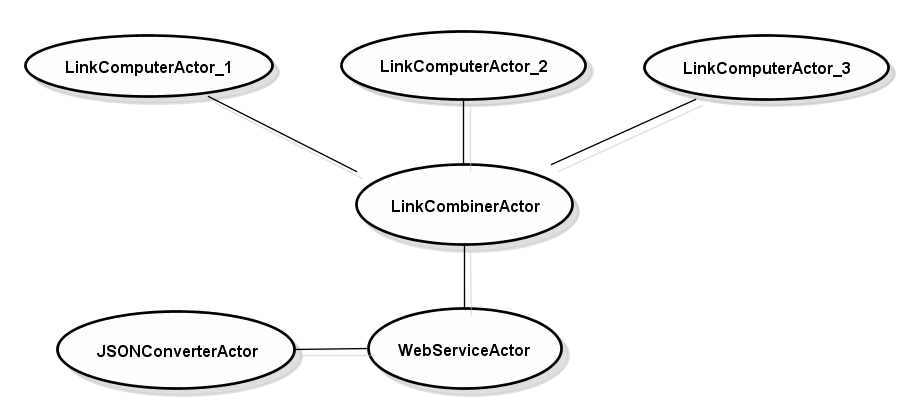
\includegraphics[width=1.00\textwidth]{ActorSystemSample}
    \caption{Simple computation actor system}
    \label{fig:actor_sample}
\end{figure}

\begin{figure}[htb]
    \centering
    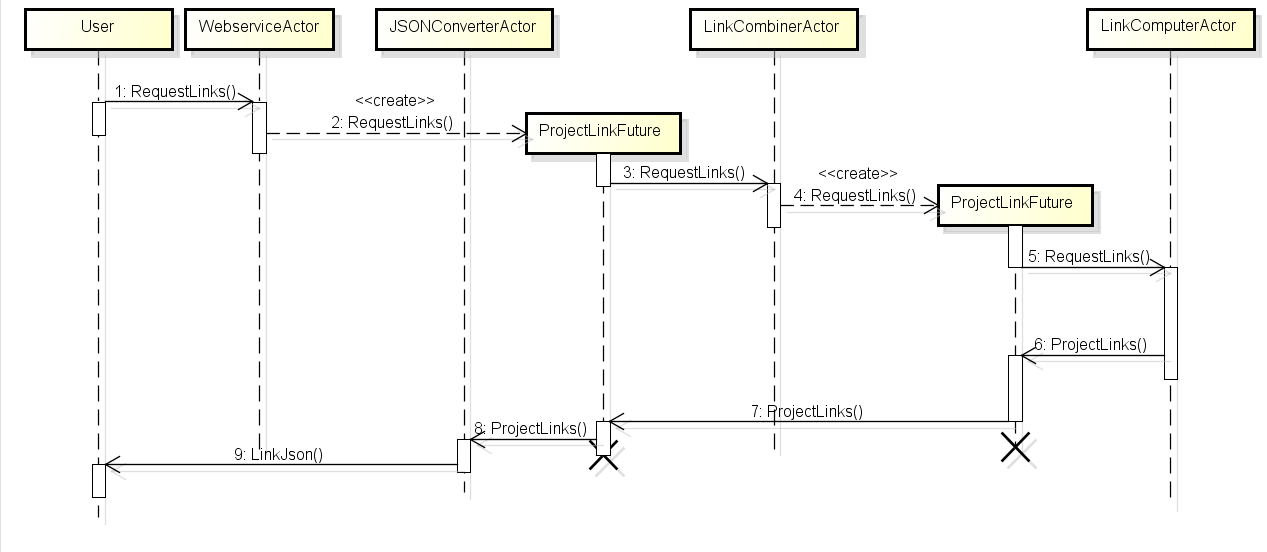
\includegraphics[width=1.0\textwidth]{ActorSequence}
    \caption{A sequence diagram for a project link request}
    \label{fig:actor_seq}
\end{figure}


When looking at figure \ref{fig:actor_seq} it is very nice to see the "WebserviceActor" and the "LinkCombinerActor" only just initiate the process. As described above the result of a request is stored in a future, and the result is piped to a new actor. This means after they receive the request both the "WebserviceActor" and the "LinkCombinerActors" are not involved in the process any more. The communication flows through the Future's they initiated.


\subsection{Scalability}

A big advantage of the design of the actor system is the scalability. Off course more LinkComputerActors can be used by the single combiner actor in figure \ref{fig:actor_sample}, but that would mean a lot of project links to be send to the same actor, resulting a lot of data flow at a single actor. 

As can be seen in the sequence diagram, both the "LinkCombineActor" and the "LinkComputerActor" can receive a project-link request. Because the actors are completely independent, they do not need to know how the project links are obtained. Therefore both actors can be substituted for each other, as shown in figure \ref{fig:example_scalable}. By doing so a tree can be constructed with link combiners and link computers, and each link computer will reduce the project-links of the next level in the tree. This way the system can be scaled into any desired size.

We have not tested the speedup of the system by using the distributed actor system at this moment. We expect a positive effect on the responsiveness of the system, but have no data yet to support this.

\begin{figure}[htb]
    \centering
    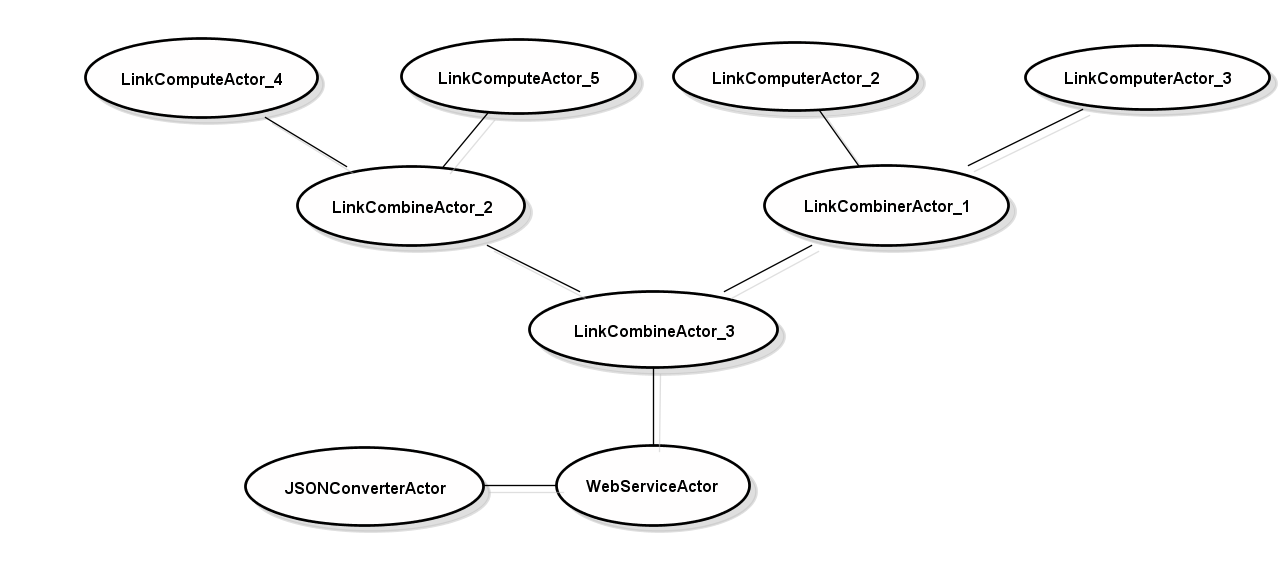
\includegraphics[width=1.00\textwidth]{ActorSystemSampleExtended}
    \caption{Example of an extended actor system}
    \label{fig:example_scalable}
\end{figure}

\section{Visualization in the browser with D3}\label{sec:visualization}

Finally, when the data has been computed to links between projects, we need a way to show this data. The objective is to provide a clear way of showing the links between projects on GitHub. We also want to show the weight of a project and the weight of a link between projects. When projects are connected, they should appear close to each other, so community structures become visible.

Therefore we choose to use a force-directed graph. The different properties of our graph are visualized as following:
\begin{itemize}
    \item Nodes repulse each other, but links have a length that keeps their nodes together. Linked projects will show up close to each other and form clusters.
    \item Project weight is used as the node radius.
    \item Link weight is used as the edge width.
\end{itemize}
In order to get a good overview the navigation over the graph is also very important. In order to browse through the graph, zoom and pan operations must be supported.

The "Data Drive Documents" (aka D3\footnote{\url{http://d3js.org}}) JavaScript library provided the functionality that we needed. The library uses SVG for rendering, includes a force-directed graph layout and out-of-the-box navigation actions. The library takes a list of nodes (our projects with their weights) and a list of links (with their weights) as input for the graph. The project weight is used for the node radius, the link weight for the edge width. This results in a graph as shown in figure \ref{fig:d3-graph}.

\begin{figure}[htb]
    \centering
    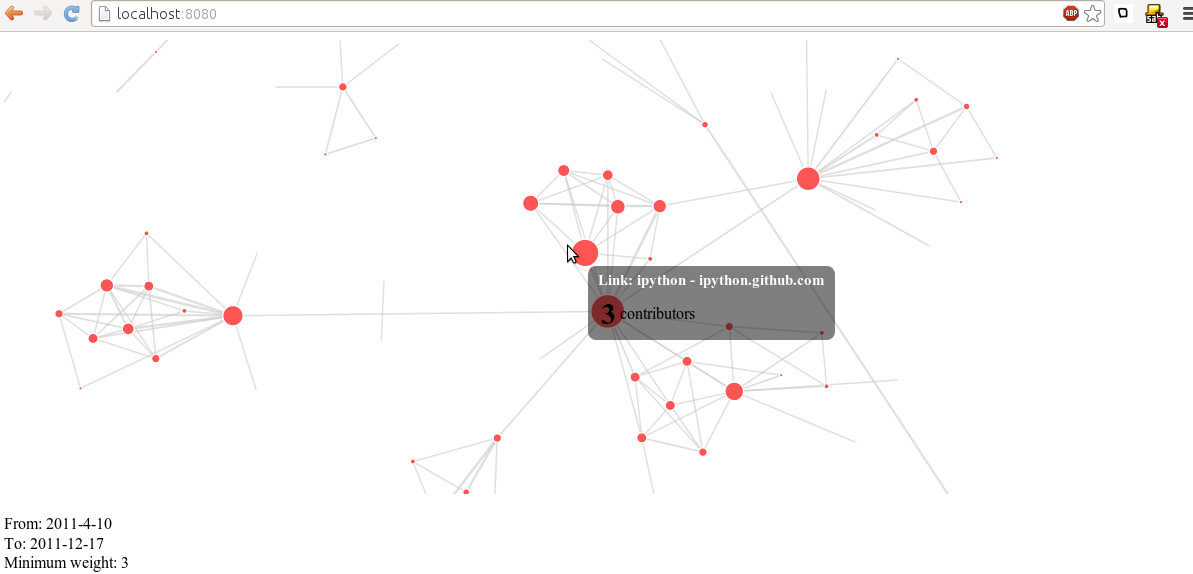
\includegraphics[width=\textwidth]{d3-graph}
    \caption{The project link graph visualized with D3}
    \label{fig:d3-graph}
\end{figure}

\section{Conclusions and suggestions}\label{sec:conclusions}

We successfully implement an interactive system to explore the project relations in our GitHub data set.

We implemented the Sawzall aggregator model as described by L\"ammel in Scala. Our implementation is more liberal then the presented one because of the use of aggregators instead of Monoids on every level of nested types. The resulting library and the integration with the Scala collections allow us to specify data processing in a very clean and elegant way.

By using Akka the computation can be distributed over multiple actor systems running on different machines. The distributed system is also scalable, ensuring that when the data size increases the system can be scaled along. We expect the distribution will have a positive effect on the responsiveness of the system, so that users can interactively query the data with different parameters without having to wait too long for the result.

With D3 as graphical library and the force directed graph, projects can be clustered together based on their links, giving a clear overview of the relation between the projects. D3 also allows easy navigation and zooming over large graphs.

Based on our experience we offer the following suggestions for future research and development:

\begin{itemize}
    \item We believe the data-processing approach as well as the visualisation library can be easily adapted for visualising other aspects of the data. It would be interesting to see this happen.
    \item It is also interesting to look at the relations of a single project. Filtering the graph for nodes that can be reached from the initial project can show the network of the project evolves over time.
    \item When the parameters are changed, the whole graph is rebuild. An approach where the graph is morphed to its new shape would be better to show evolution of networks and clusters in time.
\end{itemize}

\bibliographystyle{abbrvnat}
\bibliography{github-relations-viz}

\end{document}
